\subsection{Recovery of the Schwarzschild Metric}
  \label{subsec:recovery-of-the-schwarzschild-metric}

  In the presence of a static and approximately spherically symmetric distribution of
  localized projected configurations, the collective reduction of admissible relaxation
  ordering admits a particularly simple effective description.
  In the weak-constraint and quasi-static regime, spatial variations of the effective
  ordering rate are governed by a Poisson-like relation linking an effective potential
  to the density of localized projected configurations.

  When a geometric parametrization becomes applicable, this structure is compactly
  summarized by an effective metric whose leading-order form coincides with the
  Schwarzschild solution of general relativity.
  In this description, the temporal component encodes the local reduction of admissible
  relaxation ordering (interpreted as gravitational time dilation), while the radial
  component reflects the corresponding modulation of correlation efficiency in the spatial sector.
  The angular part of the metric follows from the approximate isotropy of the projected configuration.

  Within this framework, the standard weak-field predictions of general relativity are
  recovered, including gravitational redshift, light deflection, and time dilation in
  agreement with solar-system observations.
  The gravitational constant \(G\) appears here as an emergent collective coupling
  parameter, relating the effective density of localized projected configurations to
  the magnitude of the admissible ordering slowdown.

  \paragraph{Operational potential from \texorpdfstring{$\chi$}{χ}-relaxation slowdown (weak-field limit).}
    In the projectable regime where an effective geometric parametrization applies,
    gravitational time dilation is encoded as a \emph{local slowdown} of the relaxation
    ordering rate relative to its asymptotic value far from localized excitations.
    We therefore introduce the dimensionless lapse-like factor
    \begin{equation}
      N(r) \;\equiv\; \frac{D^\chi_{\mathrm{loc}}(r)}{D^\chi_0},
      \qquad 0 < N(r)\le 1 ,
    \end{equation}
    and define an effective Newtonian potential $\Phi$ through the weak-field identification
    \begin{equation}
      \frac{D^\chi_{\mathrm{loc}}}{D^\chi_0} \;\simeq\; 1 + \frac{\Phi}{c^2},
      \qquad \left|\frac{\Phi}{c^2}\right|\ll 1.
      \label{eq:phi_from_slowdown}
    \end{equation}
    This relation summarizes how localized projected configurations reduce admissible
    relaxation ordering, in a form directly comparable with standard gravitational phenomenology.

  \paragraph{Poisson-like equation and exterior solution.}
    In the weak-structure regime (small internal gradients compared to the saturation scale),
    coarse-graining the constrained relaxation dynamics yields the effective elliptic relation
    \begin{equation}
      \nabla^2 \Phi \;\simeq\; 4\pi G_{\mathrm{eff}}\,\rho ,
      \label{eq:poisson_phi}
    \end{equation}
    where $\rho$ is the density of localized relaxation-resistant projected configurations and
    $G_{\mathrm{eff}}$ is an emergent collective coupling. :contentReference[oaicite:2]{index=2}
    For an isolated spherically symmetric source of total mass $M$,
    the exterior solution ($r$ outside the source support) is therefore
    \begin{equation}
      \Phi(r) \;\simeq\; -\frac{G_{\mathrm{eff}} M}{r}.
      \label{eq:phi_point_mass}
    \end{equation}

  \paragraph{Metric components from \texorpdfstring{$\Phi$}{Φ} (explicit weak-field matching).}
    Once an effective geometric description becomes applicable, the metric is not postulated
    as a fundamental field equation solution; it is introduced as a compact operational encoding
    of how the slowdown factor $N(r)$ modulates proper-time accumulation and spatial correlation
    efficiency. Consistency with the interpretation of $N(r)$ as the local time-dilation factor
    implies the standard static spherically symmetric ansatz
    \begin{equation}
      ds^2 = -N(r)^2 c^2 dt^2 + N(r)^{-2} dr^2 + r^2 d\Omega^2.
      \label{eq:metric_from_N}
    \end{equation}
    In the weak-field limit, using \eqref{eq:phi_from_slowdown} gives
    \begin{align}
      g_{tt} &\simeq -\left(1 + 2\frac{\Phi}{c^2}\right),
      \label{eq:weak_gtt}\\
      g_{rr} &\simeq \left(1 + 2\frac{\Phi}{c^2}\right)^{-1}
      \;\simeq\; 1 - 2\frac{\Phi}{c^2},
      \label{eq:weak_grr}
    \end{align}
    which coincides with the standard weak-field expansion of the Schwarzschild metric after
    substituting \eqref{eq:phi_point_mass}:
    \begin{equation}
      g_{tt} \simeq -\left(1-\frac{2G_{\mathrm{eff}}M}{c^2 r}\right),
      \qquad
      g_{rr} \simeq \left(1-\frac{2G_{\mathrm{eff}}M}{c^2 r}\right)^{-1}.
      \label{eq:schwarzschild_matching}
    \end{equation}
    Equivalently, one may define the operational Schwarzschild radius by weak-field matching
    \begin{equation}
      r_s \;\equiv\; \frac{2G_{\mathrm{eff}}M}{c^2},
    \end{equation}
    so that $N(r)^2 = 1-r_s/r$ reproduces the standard Schwarzschild form at leading order. :contentReference[oaicite:3]{index=3}

    These results establish the recovery of the Schwarzschild metric as the natural
    effective description of relaxation slowdown around isolated projected configurations.

  \paragraph{Comparison to classic observational tests (weak-field regime).}
    \emph{Gravitational redshift.}
    From \eqref{eq:weak_gtt}, clock rates satisfy
    \begin{equation}
      \frac{\nu_{\mathrm{obs}}}{\nu_{\mathrm{emit}}}
      = \sqrt{\frac{-g_{tt}(r_{\mathrm{obs}})}{-g_{tt}(r_{\mathrm{emit}})}}
      \;\simeq\;
      1 + \frac{\Phi(r_{\mathrm{emit}})-\Phi(r_{\mathrm{obs}})}{c^2},
    \end{equation}
    which is the standard redshift formula tested by laboratory experiments and routinely
    accounted for in satellite navigation systems.

    \emph{Light deflection.}
    In Cosmochrony, light propagation may be described (in the projectable regime) as following
    wavefronts of constant $\chi$; equivalently, one may introduce an effective refractive index
    whose weak-field expansion yields the standard deflection angle
    \begin{equation}
      \alpha \;\simeq\; \frac{4G_{\mathrm{eff}}M}{b c^2},
    \end{equation}
    with $b$ the impact parameter, matching the general-relativistic prediction used in
    solar-system lensing and high-precision astrometry. :contentReference[oaicite:4]{index=4}

    Importantly, the Schwarzschild metric is not postulated as a fundamental solution, nor
    is spacetime curvature treated as a primitive dynamical entity.
    The metric functions instead as a compact and operational summary of how localized
    projected configurations constrain admissible relaxation ordering in their vicinity.

    Schwarzschild-like behavior therefore does not reflect a specific dynamical law of
    spacetime itself.
    It emerges as the necessary phenomenological description in regimes where projected
    configurations are close to local equilibrium and admit a smooth geometric
    representation.

    \begin{figure}[htbp]
      \centering
      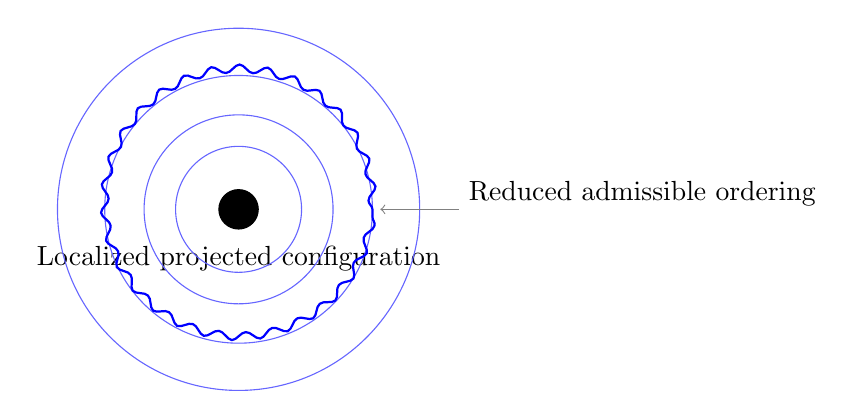
\begin{tikzpicture}[scale=1]

% Central mass
        \filldraw[black] (0,0) circle (0.25);
        \node[below] at (0,-0.35) {Localized projected configuration};

% Effective ordering contours
        \foreach \r in {0.8,1.2,1.7,2.3} {
          \draw[blue!60] (0,0) circle (\r);
        }

% Distortion
        \draw[blue, thick, decorate, decoration={snake, amplitude=0.5mm}]
        (0,0) circle (1.7);

% Arrows
        \draw[->, gray] (2.8,0) -- (1.8,0);
        \node[right] at (2.8,0.2) {Reduced admissible ordering};

      \end{tikzpicture}
      \caption
      {Emergence of Schwarzschild-like behavior in Cosmochrony.
      A localized projected configuration induces a spatially varying reduction of admissible relaxation ordering.
      In effective geometric descriptions, this manifests as differential proper-time
      accumulation and an emergent metric curvature analogous to gravitational time dilation.}
      \label{fig:chi_gravity}
    \end{figure}
